\subsection{Mixed Reality in der Lehre}
\label{sec-2-2}
\fbox{
\parbox{\linewidth}{
	\textit{Ziel des Kapitels:}\\
	State of the Art in der Überschneidung mit dem Education Bereich vorstellen.\\[6px]
	\textit{Inhalte:}
	\begin{itemize}
		\item Aktueller Einsatz von MR, insb. der HoloLens, in der Physik
		\item Einsatz von MR in Lehre allgemein, nur relevante Aspekte
	\end{itemize}
	
	\textit{Wichtige Literatur:}	
	\begin{itemize}
		\item \cite{Buchau09}
		\item Experimenting with electromagnetism using augmented reality: Impact on flow student experience and educational effectiveness Ibanez \cite{Ibanez14}
		\item Influences of AR-Supported Simulation on Learning Effectiveness in Face-to-face Collaborative Learning for Physics \cite{Li11}
		\item Real Time Simulation Method of Magnetic Field for Visualization System With Augmented Reality Technology \cite{Matsutomo13}
		\item Physics holo.lab learning experience: using smartglasses for augmented reality labwork to foster the concepts of heat conduction \cite{Strzys18}
		\item Using Augmented Reality for Teaching Physics \cite{Techakosit15}
		\item HolOsci: Hololens Augmented Reality Oscilloscope Based Support for Debugging Electronics Circuits \cite{Javaheri18}
		\item PhET: Simulations that enhance learning \cite{Wieman08}
	\end{itemize}
}}\\

Ausbildung und Training sind ein wichtiges Anwendungsgebiet für Mixed Reality Technologie. Das gilt besonders für den Bereich der Augmented Realit. In der Literatur findet sich ein breites Spektrum an Arbeiten zum Einsatz von AR zur Vermittlung von Lerninhalten und zum Training. Einige Arbeiten beleuchten die Anwendung von AR aus dem Gesichtspunkt der Lerntheorie, Psychologie und Kognitionsforschung \cite{Marichal17, Santos14}. Andere nähern sich dem Thema aus Sicht konkreter Anwendungsbeispiele und stellen speziell entwickelte AR-Lösungen vor \cite{Strzys17, Amiraslanov18, Buchau09}. Außerdem gibt es eine Reihe von Studien zu den Auswirkungen von AR-Technologie auf das Lernverhalten, den Lernerfolg und die Nutzererfahrung \cite{Ibanez14, Li11, Jerry10, Akcayir16, Strzys18}. Einen Überblick über die Forschung zum Einsatz von AR bei Lernanwendungen geben unter anderem die Arbeiten von Bacca et. al. und Chen et. al. \cite{Chen2017, Bacca14}.\\

\subsubsection{Einsatz von AR in der Lehre}
Eine umfassende Betrachtung der Hintergründe von Lerntheorien wie z.B. Multimedia Learning würde den Rahmen dieser Arbeit sprengen. Daher soll im Folgenden nur kurz auf einige Aspekte hingewiesen werden, die in bestehenden Arbeiten herausgearbeitet wurden. 

\textit{Currently, ARLEs have a mean effect size of 0.56 to stu- dent performance with wide variability due to the many possible ways to use AR, as well as, differences in experi- mental design.} \cite{Santos14}

\vspace{4px}
\textit{Hintergründe aus der Lerntheorie}\\
\textit{Cognitive offloading refers to the possibility of lightening these cognitive demands by the inclusion of actual objects representing abstract concepts. Since these objects are avail- able to the perceptual system they release working memory load} \cite{Marichal17}

\textit{1. Real world annotation improves perception. It juxtaposes real objects, and virtual text and other symbols. This reduces cognitive load in the limited working memory so that a bigger fraction of the STM can be used for operating cognitive processes (e.g., storing in the LTM).
2. Contextual visualization improves elaboration. ARLEs provide more meaningful cues found in the real environment that help a student construct a more elaborate network of knowledge.
3.
Vision-haptic visualization improves elaboration based on embodied imaging. It presents visual information in two modalities: sense of sight and sense of touch.} \cite{Santos14}

\textit{Embodied interactions with science content and new technologies with tangible and gesture-controlled interfaces have started to show enhanced learning effects. This includes environments where the body is cued to enact certain actions and create physical representations that facilitate conceptual understanding. The design rationale is that having learners act out and physicalize the systems, processes, relationships, etc., that they are trying to understand as opposed to externally manipulating these systems and processes (e.g., with a computer mouse) will create conceptual anchors from which new knowledge can be built. Up to this point, there has been little research examining outcomes for students learning the same science content in the same simulation environment, differing only in the degree of immersion and physical interaction with the interface.} \cite{Li11}


We suggest developing MR applications that enable learners to actually see and understand the fundamental facts. Specialized sensors can measure environmental data or the current status of an experiment. Voltage and current could be directly displayed within the wires during electrical engineering classes (Beheshti et al., 2017) or heat propagation in metals within physic classes (M. P. Strzys et al., 2018). MR displays in combination with sensors allows us to extend the human vision and visualize in-depth details of learning material in place of occurrence.

Once deployed, MR systems can overcome this limitation and enhance learning. In addition, interactive learning and exploring environments can be created that extend the current body of learning material. We envision interactive experiments that were not possible to realize before because of time, financial, or security constraints. For example, chemistry students could safely explore chemical reactions with hazardous elements or biology students can examine samples under an augmented micro- scope that are usually not accessible.


\textit{design strategies such as enabling exploration, promoting collaboration, and ensur- ing immersion to create compelling learning experiences.}\cite{Knierim18}


\subsubsection{In der Physik}

\vspace{4px}
\textit{holo.lab}\\
Strzys et. al. stellen eine Arbeit vor, in der eine Mixed Reality Anwendung mit der HoloLens im Kontext eines physikalischen Laborversuches genutzt wird \cite{Strzys17}. Dabei handelt es sich um ein Experiment aus der Thermodynamik, bei dem ein Metallstab gleichzeitig von der einen Seite erhitzt und von der anderen gekühlt wird. Nach kurzer Zeit ergibt sich über die Länge des Stabes ein Temperaturverlauf, der mit einer Infrarotkamera gemessen werden kann. Abbildung \ref{img:Strzys17} zeigt den Versuchsaufbau sowie die Szene aus Sicht eines Nutzers mit der HoloLens.\\

Die Messdaten der Infrarotkamera werden nun in Echtzeit an die HoloLens übertragen, die diese dann auf drei Arten darstellt:
\begin{enumerate}
	\item Ausgewählte, numerische Werte als Text
	\item Temperaturverlauf als Graph (zweidimensionale Darstellung)
	\item False-Color Prepräsentation als eingebettetes 3D-Modell, das den Metallstab überlagert
\end{enumerate}
Dabei hat der Nutzer die Möglichkeit, einzelne Darstellungsformen ein- und auszublenden. Die Autoren konstatieren zum Design der Anwendung:
\begin{quote}
	\textit{``The main focus of this design is to visualize the invisible and thus to extend human perception to new regimes, e.g., temperature and heat, thereby strengthening the connection between theory and experiment.\\ 
	In this realization the MR setting not only has the advantage of intrinsic contextuality, but also spatial and time contiguity which is supposed to support the learning process of the students. Moreover, the just-in-time evaluation of the data yields the possibility for the students to directly examine the process itself and the parameter involved, and immediately compare the outcome to theoretical predictions which we believe to enhance the links between theory and experiment.\\
	Under that perspective the effort to achieve possibly more exact numerical values for quantities like the thermal conductivity therefore seem to be less important in this setting. Instead, the technical support during the experimental phase will give students the possibility to thoroughly examine the relationship between cause and effect and thus deepen their physical understanding.''} \cite{Strzys17}
\end{quote}


\begin{figure}[h!]
	\centering
	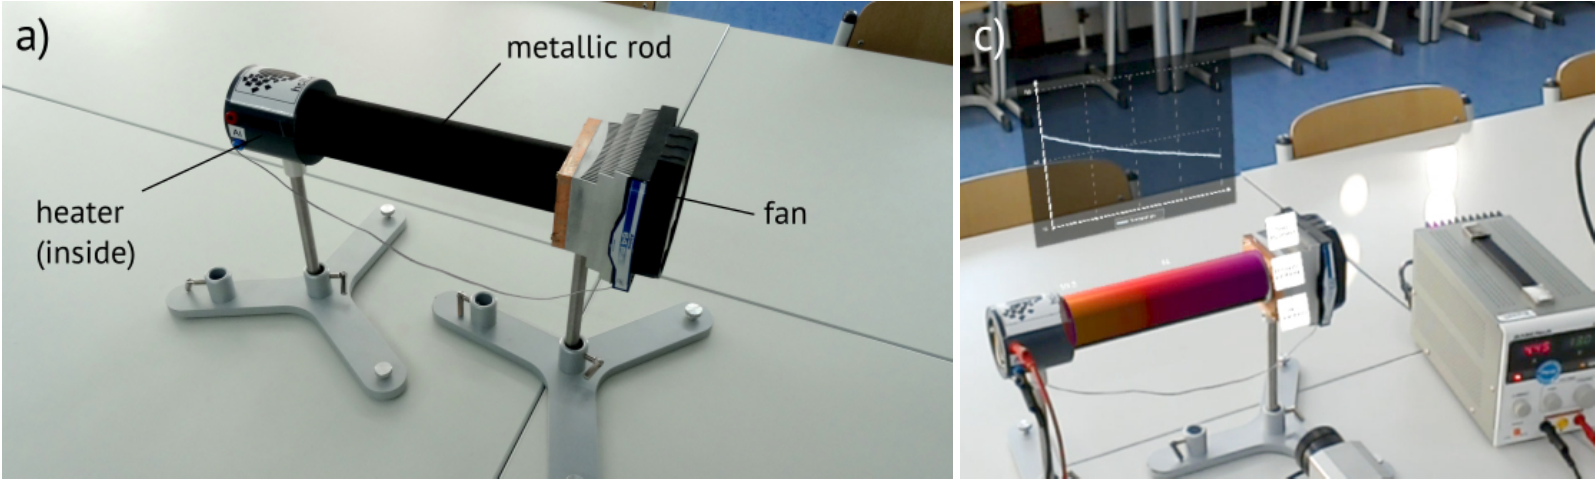
\includegraphics[width=1\textwidth]{images/Strzys18.png}
	\caption{Links: Der zu erhitzende Metallstab. Rechts: Laufendes Experiment aus Sicht eines Nutzers. \cite{Strzys17}}
	\label{img:Strzys17}
\end{figure}

\begin{figure}[h!]
	\centering
	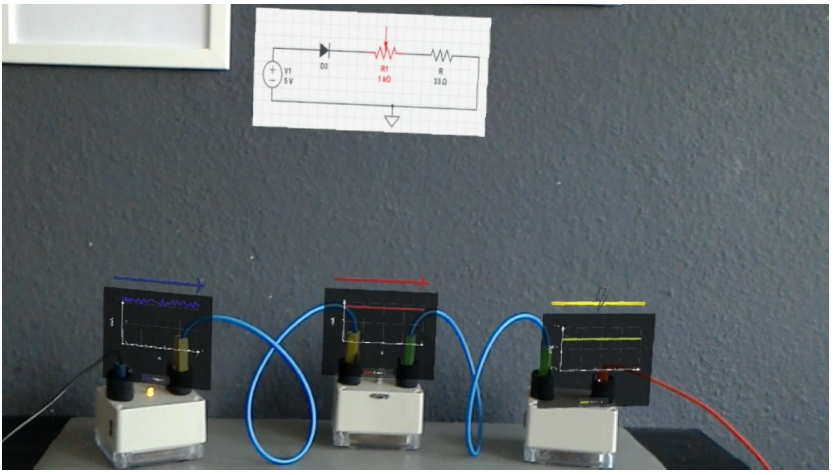
\includegraphics[width=1\textwidth]{images/Amiraslanov18.png}
	\caption{\cite{Amiraslanov18}}
	\label{img:Amiraslanov18}
\end{figure}

\begin{figure}[h!]
	\centering
	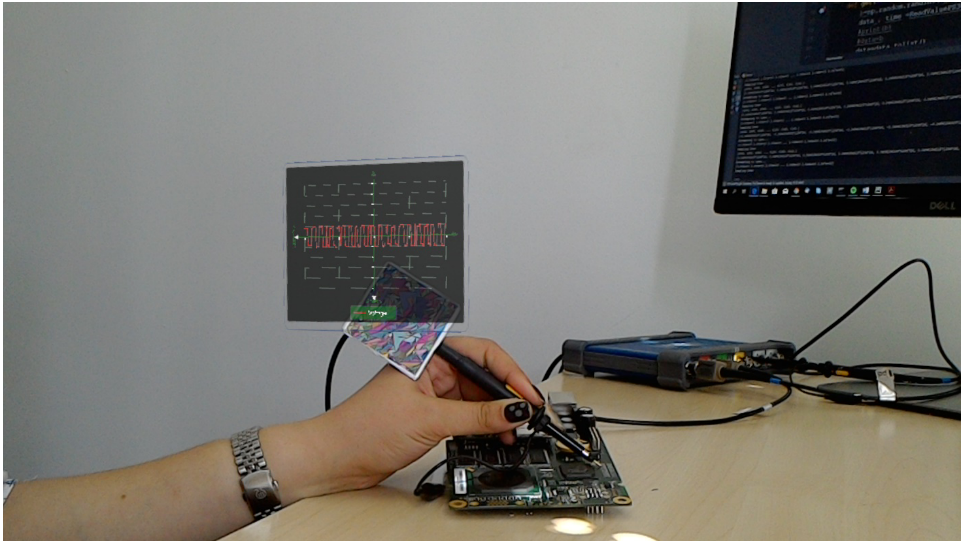
\includegraphics[width=1\textwidth]{images/Javaheri18.png}
	\caption{\cite{Javaheri18}}
	\label{img:Javaheri18}
\end{figure}

\begin{figure}[h!]
	\centering
	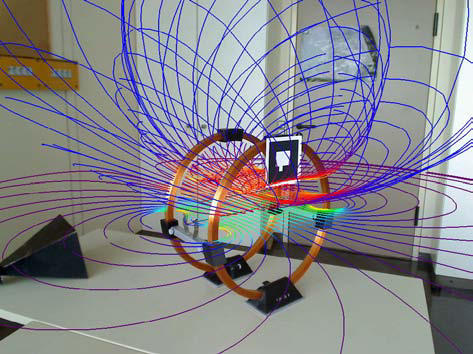
\includegraphics[width=1\textwidth]{images/Buchau09.jpg}
	\caption{\cite{Buchau09}}
	\label{img:Buchau09}
\end{figure}


\begin{itemize}
	\item AR gut geeignet für Elektromagnetismus, Darstellung von M und EM Feldern
	\item Mehrere empirische eval in der Physik, die positive Effekte zeigen
	\item mehrere aktuelle beispiele mit der HoloLens
\end{itemize}
Buchau \cite{Buchau09}, Strzys \cite{Strzys18}, Javaheri \cite{Javaheri18}, Techakosti \cite{Techakosit15} vorstellen. Weitere Arbeiten erwähnen.\\
Einordnung in Virtual Continuum und Anwendungsgebiet in der Physik.




\begin{itemize}
	\item Buchau links im AR Bereich, Magnetismus und Elektromagnetismus im Anwendungsbereich
	\item Strzys weiter rechts im AR Bereich, Thermodynamik im Anwendungsbereich
	\item Javaheri mittig im AR Bereich, Elektronik und Schaltungen im Anwendungsbereich
	\item ...
	\item ...
\end{itemize}

Fazit: So und so wird MR und HoloLens aktuell eingesetzt

